%% PyRPMD manuscript for Computer Physics Communications (CPiP article).
%% Built on the CPC elsarticle template.
\documentclass[preprint,12pt]{elsarticle}

\usepackage{amssymb}
\usepackage{amsmath}
\usepackage{graphicx}
\usepackage{booktabs}
\usepackage{tabularx}
\usepackage{array}
\usepackage{xcolor}
\usepackage{listings}
\usepackage{tikz}
\usetikzlibrary{positioning,fit,arrows.meta,backgrounds}
\usepackage[hidelinks]{hyperref}

\biboptions{sort&compress}

\lstset{basicstyle=\ttfamily\footnotesize,columns=fullflexible,keepspaces=true,
  frame=single,framerule=0.3pt,rulecolor=\color{black!40},xleftmargin=4pt,xrightmargin=4pt,
  showstringspaces=false,breaklines=true}

%% List environment for the references of the Program Summary
\newcounter{bla}
\newenvironment{refnummer}{%
\list{[\arabic{bla}]}%
{\usecounter{bla}%
 \setlength{\itemindent}{0pt}%
 \setlength{\topsep}{0pt}%
 \setlength{\itemsep}{0pt}%
 \setlength{\labelsep}{2pt}%
 \setlength{\listparindent}{0pt}%
 \settowidth{\labelwidth}{[9]}%
 \setlength{\leftmargin}{\labelwidth}%
 \addtolength{\leftmargin}{\labelsep}%
 \setlength{\rightmargin}{0pt}}}
 {\endlist}

\newcommand{\code}[1]{\texttt{#1}}
\newcommand{\kB}{k_{\mathrm{B}}}
\newcommand{\Eh}{E_{\mathrm{h}}}
\newcommand{\rateunit}{\mathrm{cm^{3}\,molecule^{-1}\,s^{-1}}}

\emergencystretch=2em
\journal{Computer Physics Communications}

\begin{document}

\begin{frontmatter}

\title{PyRPMD: a unified Python/C++ program for ring-polymer molecular dynamics --- reaction rates, direct scattering, free energies, transport and spectra}

%% TODO(authors): replace the placeholders below with the real author list,
%% affiliations and corresponding-author address before submission.
\author[a]{First Author\corref{author}}
\author[a]{Second Author}

\cortext[author]{Corresponding author.\\\textit{E-mail address:} corresponding.author@institution.edu}
\address[a]{Affiliation, City, Country}

\begin{abstract}
We present PyRPMD, an open-source program that carries a ring-polymer molecular dynamics (RPMD) calculation from a single text input to a statistically qualified observable. One code base provides restartable workflows for bimolecular thermal rate constants (Bennett--Chandler factorisation with umbrella-integration, MBAR, metadynamics or OPES potentials of mean force), direct RPMD scattering with product-channel classification, one- to three-dimensional free-energy surfaces, equilibrium path-integral molecular dynamics in the $NVT$ and $NPT$ ensembles, centroid diffusion, site-to-site and surface escape rates, and thermostatted-RPMD vibrational spectra, together with instanton, nonadiabatic and electrochemical proton-coupled electron-transfer modules. Three symplectic ring-polymer integrators are implemented twice: as C++17/OpenMP kernels that fuse the integrator, the potential call, the bias and the collective-variable observation into one compiled block, and as a NumPy reference implementation that is selectable at run time and agrees with the kernels to $10^{-11}$ in the phase-space coordinates after $10^{3}$ steps. The fused kernels advance a 128-bead triatomic ring polymer in $13~\mu$s per step, 20 times faster than the reference implementation, and independent trajectories are distributed over worker processes with bit-identical results. Every workflow shares explicit, dimension-checked units, hash-verified atomic checkpoints, a scientific identity that prevents a restart from silently changing the physics, and uncertainty estimates that respect the correlation structure of the data. We validate the program against analytic finite-bead results, exact quantum references, two independent routes to the same rate constant, and the published RPMD rate of H + H$_2$ on the BKMP2 surface, which is reproduced to within 1\%.
\end{abstract}

\begin{keyword}
ring-polymer molecular dynamics \sep path-integral molecular dynamics \sep reaction rate constants \sep nuclear quantum effects \sep free-energy calculations \sep enhanced sampling
\end{keyword}

\end{frontmatter}

{\bf PROGRAM SUMMARY}

\begin{small}
\noindent
{\em Program Title:} PyRPMD \\
{\em CPC Library link to program files:} (to be added by Technical Editor) \\
{\em Developer's repository link:} \url{https://github.com/chen-yu-hao/PyRPMD} \\
{\em Code Ocean capsule:} (to be added by Technical Editor)\\
{\em Licensing provisions:} MIT \\
{\em Programming language:} Python 3.11+ and C++17 (OpenMP); optional C and Fortran potential libraries through a versioned C ABI \\
{\em Supplementary material:} User manual in English and Chinese, analytic tutorial inputs with comparison scripts, and the scripts and data records that regenerate every figure and table of this article. \\
{\em Nature of problem:}\\
Nuclear quantum effects --- zero-point energy and tunnelling --- change thermal rate constants, free energies, diffusion coefficients and vibrational spectra of systems containing light atoms by amounts that classical molecular dynamics cannot capture. Ring-polymer molecular dynamics (RPMD) [1,2] includes them at the cost of classical trajectories in an extended phase space, but a quantitative RPMD observable is the end product of a long chain of coupled steps: preparation of a transition state and reaction coordinate, biased sampling, free-energy reconstruction, constrained sampling of a dividing surface, real-time recrossing dynamics, normalisation and error analysis. Each observable has so far required its own program and its own conventions for units, normalisation and restart, which makes cross-validation between methods laborious and results difficult to reproduce. \\
{\em Solution method:}\\
PyRPMD represents every calculation as a validated job specification executed by a restartable workflow on top of one propagation stack. The ring-polymer Hamiltonian is integrated with the Cayley BCB [3], exact normal-mode BAB or velocity-Verlet splitting, combined with Andersen, PILE, stochastic-velocity-rescaling, Nos\'e--Hoover-chain, generalised-Langevin or PIGLET thermostats and with isotropic barostats. Compiled C++17/OpenMP kernels execute whole propagation blocks, including the potential, the bias, constraints and collective-variable observations, without returning to the interpreter; an equivalent NumPy implementation serves as the numerical reference. Thermal rates are obtained from the Bennett--Chandler factorisation [4], $k=\kappa\,k_{\mathrm{QTST}}$, with the centroid potential of mean force from umbrella integration, a streaming MBAR solver, well-tempered metadynamics or OPES, and with the transmission coefficient from paired unbiased child trajectories launched from RATTLE-constrained parents; the same rate is available independently from direct RPMD collisions. Statistical errors are propagated by block and parent-cluster bootstraps. Potentials are attached through a batched interface with adapters for Python, C/C++/Fortran, ASE, OpenMM, LAMMPS, i-PI, PyTorch and machine-learning models. \\
{\em Additional comments including restrictions and unusual features:}\\
All inputs carry explicit units that are checked for dimension. Checkpoints are written atomically, store a SHA-256 inventory of their arrays and are bound to a fingerprint of the scientific input, so that an interrupted calculation resumes on the same random streams and a changed Hamiltonian is refused. Rates are released only when the recrossing plateau and energy-conservation diagnostics pass. Execution is serial, multi-process, MPI (trajectory $\times$ bead topology) or batched on GPUs through PyTorch potentials; the result of a calculation is independent of the number of workers. The program requires only NumPy, SciPy, h5py and threadpoolctl; all other interfaces are optional.

\begin{thebibliography}{0}
\bibitem{ps1} I. R. Craig, D. E. Manolopoulos, J. Chem. Phys. 121 (2004) 3368.
\bibitem{ps2} S. Habershon, D. E. Manolopoulos, T. E. Markland, T. F. Miller III, Annu. Rev. Phys. Chem. 64 (2013) 387.
\bibitem{ps3} R. Korol, N. Bou-Rabee, T. F. Miller III, J. Chem. Phys. 151 (2019) 124103.
\bibitem{ps4} R. Collepardo-Guevara, Y. V. Suleimanov, D. E. Manolopoulos, J. Chem. Phys. 130 (2009) 174713.
\end{thebibliography}
\end{small}

%% ===================================================================
\section{Introduction}
\label{sec:introduction}

Light nuclei are quantum objects at ordinary temperatures. Zero-point energy and tunnelling shift the rate constants of hydrogen-transfer reactions by orders of magnitude at low temperature, reorder kinetic isotope effects, change the structure and transport properties of hydrogen-bonded liquids and of hydrogen in metals, and redistribute intensity in vibrational spectra \cite{markland2018}. Imaginary-time path integrals map the quantum statistics of $N$ distinguishable nuclei exactly onto the classical statistics of a ring polymer of $P$ replicas connected by harmonic springs \cite{cw81,pr84}, and ring-polymer molecular dynamics (RPMD) uses the classical dynamics of that ring polymer as an approximation to Kubo-transformed quantum time-correlation functions \cite{rpm04,habershon2013}. RPMD is exact in the high-temperature, short-time and harmonic limits, conserves the quantum Boltzmann distribution, and yields rate constants that are rigorously independent of the choice of dividing surface \cite{rate05,rate05b}. Because it costs only $P$ times a classical trajectory and applies without modification in full dimensionality, it has become the method of choice for thermal rate constants of polyatomic gas-phase reactions \cite{bimol09,suleimanov2016}, and it is used equally for diffusion in liquids and solids, for adsorbate dynamics on surfaces and, in its thermostatted form \cite{trpmd14}, for vibrational spectroscopy.

Turning this simple idea into a number with an error bar is a different matter. A thermal rate constant from the Bennett--Chandler procedure \cite{bennett1977,chandler1978,bimol09} requires a transition-state geometry and a reaction coordinate that interpolates between the reactant asymptote and the barrier, tens to hundreds of biased ring-polymer simulations, a free-energy reconstruction, a long constrained simulation on the dividing surface, thousands of unbiased real-time trajectories, the correct bimolecular normalisation, and an error analysis that accounts for the correlation between all of these stages. A diffusion coefficient, a free-energy surface or a spectrum has its own chain of comparable length. The established programs each cover a part of this landscape with great success: RPMDrate \cite{rpmrate13} automates gas-phase bimolecular rates for analytic potential-energy surfaces, i-PI \cite{ipi2014,ipi2019} provides a universal client--server force engine for path-integral sampling and dynamics, and general molecular-dynamics packages such as OpenMM \cite{openmm2017} and LAMMPS \cite{lammps1995} expose ring-polymer integrators. A researcher who wants to compare a Bennett--Chandler rate with a direct-scattering rate on the same surface, to carry a gas-phase protocol over to a reaction at a surface, or to replace an analytic potential by a machine-learned one must nevertheless move between programs with different units, different normalisation conventions and incompatible restart files, and must assemble the statistical analysis by hand.

PyRPMD removes these seams. It is a single program in which \emph{(i)} one validated input file selects the observable, \emph{(ii)} one propagation stack advances the ring polymer for every observable, \emph{(iii)} one batched potential interface serves analytic, compiled, \emph{ab initio} and machine-learned surfaces alike, and \emph{(iv)} one checkpoint and identity mechanism makes every stage of every workflow restartable and auditable. Its contributions are the following.

\begin{itemize}
\item \textbf{End-to-end workflows for the principal RPMD observables.} Bimolecular rate constants, direct collision outcomes, free-energy surfaces, equilibrium path-integral averages, diffusion coefficients, first-order site and surface rates and vibrational spectra are all produced by the same four commands (\code{validate}, \code{run}, \code{analyze}, \code{resume}) from the same input grammar.
\item \textbf{Two independent routes to a rate constant in one program.} The Bennett--Chandler rate and the direct RPMD (dRPMD) collision rate \cite{drpmd18} share the potential, the integrator and the normalisation, so that the agreement of two estimators with entirely different statistical structure becomes a routine internal check (Section~\ref{sec:val-rates}).
\item \textbf{Fused native propagation with a reference twin.} C++17/OpenMP kernels execute complete propagation blocks --- free-ring evolution, potential, bias, constraint and observation --- without an interpreter round trip, while a NumPy implementation of the same integrators remains selectable at run time for verification. The fused path is one to two orders of magnitude faster than the reference at identical numerical results (Section~\ref{sec:performance}).
\item \textbf{A modern free-energy toolbox coupled to rate theory.} Umbrella integration, a streaming multistate Bennett acceptance ratio (MBAR) solver, adaptive window placement, replica exchange, well-tempered metadynamics and OPES all deliver potentials of mean force in the flux-weighted measure that the rate expression requires.
\item \textbf{Statistics and provenance as part of the result.} Block and parent-cluster bootstraps propagate the joint uncertainty of the free energy and of the transmission coefficient; a rate is released only when its plateau and energy diagnostics pass; and each run stores its resolved input, seeds, software versions and hash-verified checkpoints.
\item \textbf{Breadth beyond the Born--Oppenheimer ring polymer.} Ring-polymer instantons, a subspace quantum correction of RPMD rates, nonadiabatic ring-polymer methods, electronic friction, constant-potential electrode models and golden-rule proton-coupled electron transfer are available behind the same potential and unit conventions.
\end{itemize}

The remainder of this article is organised as follows. Section~\ref{sec:theory} fixes the conventions. Section~\ref{sec:architecture} describes the architecture, Section~\ref{sec:functionality} the functionality and Section~\ref{sec:usage} installation and use. Section~\ref{sec:validation} reports numerical validation, Section~\ref{sec:performance} performance, and Section~\ref{sec:advantages} summarises what the design gains over a collection of separate tools.

%% ===================================================================
\section{Theoretical background and conventions}
\label{sec:theory}

\subsection{Ring-polymer Hamiltonian}

For $N$ atoms with masses $m_i$ at inverse temperature $\beta=1/\kB T$, PyRPMD propagates the $P$-bead ring-polymer Hamiltonian in the summed convention ($\hbar=1$),
\begin{equation}
H_P(\mathbf p,\mathbf q)=\sum_{j=0}^{P-1}\left[\sum_{i=1}^{N}\frac{|\mathbf p_{ji}|^{2}}{2m_i}
+\sum_{i=1}^{N}\frac{m_i\omega_P^{2}}{2}\,|\mathbf q_{ji}-\mathbf q_{j-1,i}|^{2}+V(\mathbf q_j)\right],
\qquad \omega_P=\frac{P}{\beta},
\label{eq:hamiltonian}
\end{equation}
with cyclic bead index. The equilibrium distribution is $\exp[-(\beta/P)H_P]$; for $P=1$ the springs vanish and the dynamics is classical. The physical masses are retained, so that the time variable of an unthermostatted trajectory is physical time and the Kubo-transformed correlation function of two position-dependent operators is approximated by \cite{rpm04}
\begin{equation}
\tilde C_{AB}(t)\simeq\frac{1}{(2\pi)^{3NP}Z_P}\int\!\mathrm d\mathbf p\,\mathrm d\mathbf q\;
e^{-(\beta/P)H_P}\,\bar A(\mathbf q_0)\,\bar B(\mathbf q_t),\qquad
\bar A(\mathbf q)=\frac1P\sum_{j}A(\mathbf q_j).
\end{equation}
All internal quantities are in Hartree atomic units; positions and momenta are stored as arrays of shape $[P,N,3]$, and a potential returns the physical energy and force of each bead, to which the program adds springs, biases and constraints.

\subsection{Integrators and thermostats}

A time step is the symmetric splitting B--A--B, in which B is a half kick by the physical (and bias) forces and A evolves the free ring polymer. PyRPMD implements three realisations of A: the Cayley map of Korol, Bou-Rabee and Miller \cite{cayley19}, which is strongly stable for every ring-polymer frequency and is the default; the exact normal-mode rotation \cite{pile10}; and explicit velocity Verlet \cite{vv82}. For sampling, the Ornstein--Uhlenbeck step O is inserted as BCOCB \cite{bcocb20} with the Cayley map or as BAOAB \cite{baoab13} with the exact rotation. The available heat baths are Andersen collisions \cite{and80}, the path-integral Langevin thermostats PILE-L and PILE-G \cite{pile10}, stochastic velocity rescaling \cite{svr07}, Nos\'e--Hoover chains \cite{nhc92}, generalised Langevin equations including PIGLET \cite{gle09,piglet12} and fast-forward Langevin \cite{ffl18}. Isotropic constant-pressure sampling uses the Bussi--Zykova--Parrinello and Martyna--Tobias--Klein families of barostats \cite{bzp2009,mtk1994}. Holonomic constraints are imposed by SHAKE and RATTLE \cite{shake77,rattle83}; the constraint of the centroid to a dividing surface, which the rate workflow needs, is a centroid RATTLE compatible with the Cayley map. Ring-polymer contraction \cite{rpc08} and multiple time stepping \cite{respa92,mts16} are expressed as an explicit splitting of the potential into fast and slow parts.

\subsection{Thermal rate constants}

For a bimolecular reaction $\mathrm A+\mathrm B\to$ products the RPMD rate constant is written in Bennett--Chandler form \cite{bimol09},
\begin{equation}
k_{\mathrm{RPMD}}(T)=\kappa(t\to t_{\mathrm p})\,k_{\mathrm{QTST}}(T;\xi^{\ddagger}),
\label{eq:bc}
\end{equation}
where $\xi(\bar{\mathbf q})$ is a dimensionless function of the centroid $\bar{\mathbf q}$ that equals $0$ on a dividing surface in the reactant asymptote (centre-of-mass separation $R_\infty$) and $1$ on a surface through the transition state \cite{rpmrate13}. The static factor is the centroid-density quantum transition-state-theory rate,
\begin{equation}
k_{\mathrm{QTST}}=4\pi R_\infty^{2}\left(\frac{1}{2\pi\beta\mu_R}\right)^{1/2}
e^{-\beta\,[W(\xi^{\ddagger})-W(0)]},
\label{eq:qtst}
\end{equation}
with $\mu_R$ the reduced mass of the reactants and $W(\xi)$ the potential of mean force in the flux-weighted measure $\delta(\xi-\xi(\bar{\mathbf q}))\,[\nabla\xi\cdot\mathbf M^{-1}\nabla\xi/2\pi\beta]^{1/2}$. The dynamical factor is the plateau value of the ring-polymer transmission coefficient,
\begin{equation}
\kappa(t)=\frac{\langle \delta(\xi_0-\xi^{\ddagger})\,\dot\xi_0\,h(\xi_t-\xi^{\ddagger})\rangle}
{\langle \delta(\xi_0-\xi^{\ddagger})\,\dot\xi_0\,h(\dot\xi_0)\rangle},
\label{eq:kappa}
\end{equation}
evaluated from unbiased trajectories that start on the dividing surface. The product of Eqs.~(\ref{eq:qtst}) and (\ref{eq:kappa}) is independent of $\xi^{\ddagger}$. Local first-order processes --- a hop between interstitial sites or the escape of an adsorbate from a surface basin --- use the same factorisation with the bimolecular prefactor replaced by an explicit basin probability, and yield rates in $\mathrm s^{-1}$.

The same bimolecular rate is the thermal average of the reactive flux through the entrance channel. In direct RPMD \cite{drpmd18} thermalised ring polymers of the two reactants are launched towards each other with relative energy $E\sim\mathrm{Gamma}(2,\kB T)$ and impact parameter uniform in $b^{2}\le b_{\max}^{2}$, and
\begin{equation}
k_{\mathrm{dRPMD}}=\left(\frac{8}{\pi\beta\mu_R}\right)^{1/2}\pi b_{\max}^{2}\;\frac{N_{\mathrm r}}{N_{\mathrm{traj}}},
\label{eq:drpmd}
\end{equation}
where $N_{\mathrm r}$ is the number of trajectories classified as reactive. Equations~(\ref{eq:bc}) and (\ref{eq:drpmd}) share no sampling stage, no free-energy estimator and no dividing surface, which makes their comparison a stringent test of an implementation.

\subsection{Free energies and equilibrium estimators}

A free-energy surface over collective variables $\mathbf s$ is the density free energy $F(\mathbf s)=-\beta^{-1}\ln\rho(\mathbf s)+C$, with the histogram mass divided by the bin volume. A physical umbrella $w(\mathbf s)=\frac12(\mathbf s-\mathbf c)^{\mathsf T}\mathbf K(\mathbf s-\mathbf c)$ enters Eq.~(\ref{eq:hamiltonian}) as $P\,w$, so that the reduced bias in the MBAR equations \cite{samp-mbar2008} is $\beta w$ irrespective of $P$. Collective variables can be evaluated on the centroid or as bead averages; the two are distinguished in the input because they differ for nonlinear functions. Equilibrium path-integral runs report the bead-averaged potential energy and the centroid-virial kinetic energy,
\begin{equation}
K_{\mathrm{cv}}=\frac{3N}{2\beta}-\frac{1}{2P}\sum_{j,i}(\mathbf q_{ji}-\bar{\mathbf q}_i)\cdot\mathbf F_{ji},
\label{eq:kcv}
\end{equation}
the ring radius of gyration and, at constant pressure, the cell volume and the virial pressure.

%% ===================================================================
\section{Program architecture}
\label{sec:architecture}

PyRPMD is organised in five layers (Fig.~\ref{fig:architecture}). A calculation enters as a job specification and is resolved into a fully explicit configuration; a workflow decomposes it into restartable stages; every stage advances ring polymers through the common propagation stack, which calls the potential through one batched interface; the analysis layer turns the stored observations into an observable with an uncertainty.

\begin{figure}[!htbp]
\centering
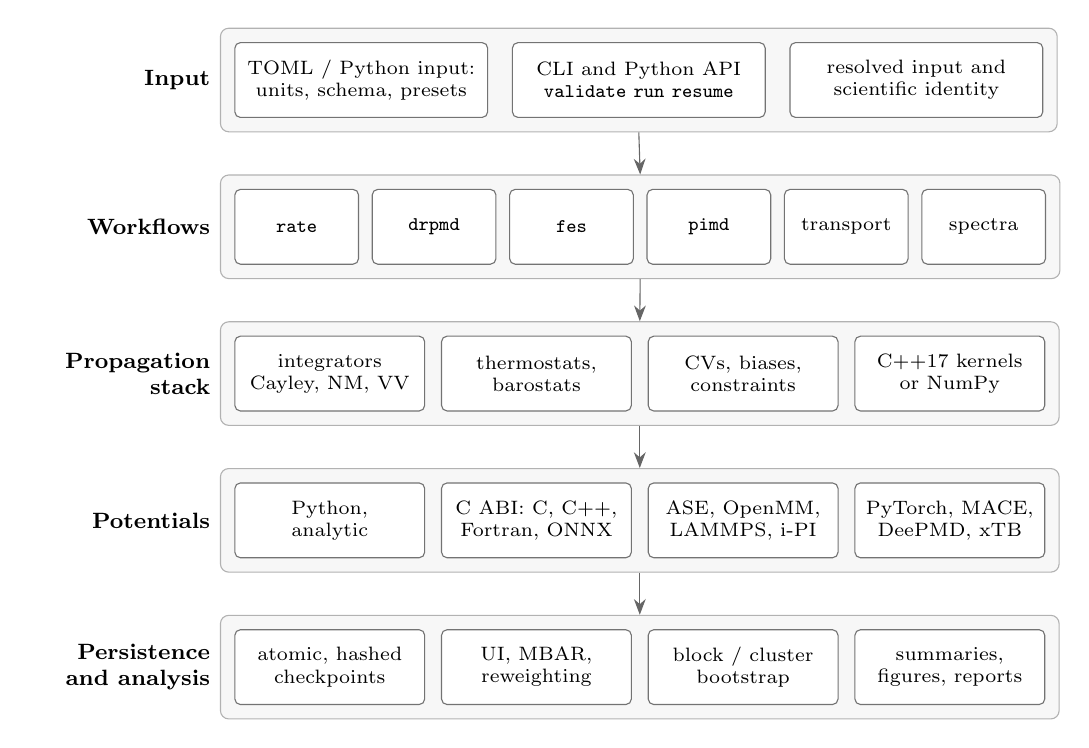
\begin{tikzpicture}[font=\footnotesize,
  box/.style={draw=black!55,rounded corners=2pt,minimum height=9.5mm,inner sep=3pt,align=center,fill=white,font=\scriptsize},
  layer/.style={draw=black!30,rounded corners=3pt,inner sep=5pt,fill=black!3},
  lab/.style={font=\footnotesize\bfseries,anchor=east,align=right,text width=22mm},
  arr/.style={-{Stealth[length=2mm]},black!60}]
\node[box,text width=30mm] (toml) {TOML / Python input:\\units, schema, presets};
\node[box,text width=30mm,right=3mm of toml] (cli) {CLI and Python API\\\code{validate run resume}};
\node[box,text width=30mm,right=3mm of cli] (id) {resolved input and\\scientific identity};
\begin{scope}[on background layer]\node[layer,fit=(toml)(cli)(id)] (L1) {};\end{scope}
\node[lab] at (L1.west) {Input};

\node[box,text width=13.6mm,below=9mm of toml.south west,anchor=north west] (rate) {\code{rate}};
\node[box,text width=13.6mm,right=1.6mm of rate] (drpmd) {\code{drpmd}};
\node[box,text width=13.6mm,right=1.6mm of drpmd] (fes) {\code{fes}};
\node[box,text width=13.6mm,right=1.6mm of fes] (pimd) {\code{pimd}};
\node[box,text width=13.6mm,right=1.6mm of pimd] (diff) {transport};
\node[box,text width=13.6mm,right=1.6mm of diff] (spec) {spectra};
\begin{scope}[on background layer]\node[layer,fit=(rate)(spec)] (L2) {};\end{scope}
\node[lab] at (L2.west) {Workflows};

\node[box,text width=22mm,below=9mm of rate.south west,anchor=north west] (int) {integrators\\Cayley, NM, VV};
\node[box,text width=22mm,right=2mm of int] (th) {thermostats,\\barostats};
\node[box,text width=22mm,right=2mm of th] (bias) {CVs, biases,\\constraints};
\node[box,text width=22mm,right=2mm of bias] (exec) {C++17 kernels\\or NumPy};
\begin{scope}[on background layer]\node[layer,fit=(int)(exec)] (L3) {};\end{scope}
\node[lab] at (L3.west) {Propagation stack};

\node[box,text width=22mm,below=9mm of int.south west,anchor=north west] (py) {Python,\\analytic};
\node[box,text width=22mm,right=2mm of py] (cabi) {C ABI: C, C++,\\Fortran, ONNX};
\node[box,text width=22mm,right=2mm of cabi] (ext) {ASE, OpenMM,\\LAMMPS, i-PI};
\node[box,text width=22mm,right=2mm of ext] (ml) {PyTorch, MACE,\\DeePMD, xTB};
\begin{scope}[on background layer]\node[layer,fit=(py)(ml)] (L4) {};\end{scope}
\node[lab] at (L4.west) {Potentials};

\node[box,text width=22mm,below=9mm of py.south west,anchor=north west] (ck) {atomic, hashed\\checkpoints};
\node[box,text width=22mm,right=2mm of ck] (mbar) {UI, MBAR,\\reweighting};
\node[box,text width=22mm,right=2mm of mbar] (boot) {block / cluster\\bootstrap};
\node[box,text width=22mm,right=2mm of boot] (rep) {summaries,\\figures, reports};
\begin{scope}[on background layer]\node[layer,fit=(ck)(rep)] (L5) {};\end{scope}
\node[lab] at (L5.west) {Persistence and analysis};

\draw[arr] (L1.south) -- (L2.north);
\draw[arr] (L2.south) -- (L3.north);
\draw[arr] (L3.south) -- (L4.north);
\draw[arr] (L4.south) -- (L5.north);
\end{tikzpicture}
\caption{Layered architecture of PyRPMD. Every workflow uses the same propagation stack, potential interface and persistence layer; process, MPI and trajectory-batching executors (not shown) distribute independent stages across resources.}
\label{fig:architecture}
\end{figure}

\subsection{Job specification and preflight}

An input is a TOML file or a Python module that builds the same mapping. Dimensional quantities are strings with units (\code{"0.1 fs"}, \code{"300 K"}, \code{"0.7 eV"}, \code{"0.004 hartree/bohr\^{}2"}) that are parsed and checked for dimension; unknown fields and fields that belong to an inactive method are rejected, so that a misspelt option cannot be ignored silently. \code{pyrpmd validate} resolves the input into a complete configuration, reports the execution backend planned for each stage, constructs the potential on request (\code{--check-pes}) and probes MPI, GPU and optional libraries without starting a calculation. The resolved configuration can be written out and is stored with the run.

\subsection{Potential interface}

A potential is an object with one method that maps coordinates of shape $[B,N,3]$ (bohr) to energies $[B]$ and forces $[B,N,3]$, with an optional virial and a per-structure status, where $B$ is the number of structures in the call. The batch dimension is what allows the same interface to serve a loop over beads in a Fortran routine, a vectorised NumPy function, a pool of \emph{ab initio} clients and a single forward pass of a neural network over all beads of many trajectories. Adapters convert units and derivative conventions on the boundary. The built-in adapters cover analytic models; arbitrary Python factories; a versioned C ABI for C, C++ and Fortran \code{BIND(C)} libraries, whose second version adds cells, periodic boundary conditions and virials; legacy RPMDrate/f2py surfaces; ASE calculators \cite{ase2017}; OpenMM \cite{openmm2017} and LAMMPS \cite{lammps1995}; a persistent i-PI client pool \cite{ipi2014}; batched PyTorch models \cite{torch2019}; MACE, NequIP and DeePMD-kit \cite{mace2022,nequip2022,deepmd2018}; on-the-fly GFN-xTB \cite{gfn22019}; and PySCF \cite{pyscf2018}. A finite-difference checker verifies any provider before it is used.

\subsection{Propagation stack and native kernels}
\label{sec:native}

The class \code{Dynamics} composes an integrator, an optional thermostat, an optional barostat and an optional force splitting into a propagation plan. The plan is executed by one of three paths that implement identical mathematics:
\begin{enumerate}
\item \emph{Fused native blocks.} When the potential, the bias and the requested observations have a compiled representation, a block of up to 65\,536 steps runs entirely in C++ with the global interpreter lock released. The kernel reuses the end-point force of each step, so that $L$ steps cost $L+1$ potential batches; it keeps the accepted and the trial state in two buffers that are swapped by pointer, so that a failed step leaves the last accepted state intact; and it evaluates the reaction coordinate, its gradient and the metric term of the flux-weighted bias once per force call and shares them between the bias and the observation. Compiled potentials attached through the C ABI and the built-in analytic models are called directly.
\item \emph{Compiled substeps.} For potentials or biases defined in Python --- for instance a neural network or a history-dependent bias --- the time loop runs in Python while the free-ring step, the thermostat and the constraint solver remain compiled.
\item \emph{NumPy reference.} A pure NumPy implementation of every integrator serves as the numerical reference and as the fallback on platforms without a compiler.
\end{enumerate}
The path is selected per stage by \code{loop\_backend = "auto"|"native"|"python"}; \code{"native"} refuses to run rather than fall back. The backend used and the number of native and interpreted steps are recorded in every result summary. A separate persistent C++ ensemble engine drives equilibrium PIMD with the full set of thermostats and barostats; a counter-based Philox generator gives every replica its own reproducible random stream. The free-energy analysis has its own native component, a streaming MBAR solver that never materialises the states-by-samples matrix.

\subsection{Parallel execution}

RPMD workloads are dominated by independent units --- umbrella windows, parent chains, child trajectories, collisions, replicas --- and PyRPMD parallelises over these first. The process backend distributes them over local workers; the MPI backend arranges ranks in a $G\times B$ topology of $G$ trajectory groups with $B$ bead-evaluation ranks each, with static or dynamic scheduling; and trajectory batching merges the potential requests of up to 256 independent trajectories into one call, which is the efficient layout for GPU-resident machine-learned potentials. Random streams, clocks and checkpoints belong to the unit, not to the worker, so the result of a calculation does not depend on the number of workers or on the scheduling order.

\subsection{Checkpoints, identity and restart}

Every stage writes portable NPZ checkpoints through a write--flush--fsync--rename sequence, so that an interruption leaves the previous complete file in place. A checkpoint carries an inventory with the type, shape and SHA-256 digest of each array, which is verified before any state is exposed; pickled objects are never read. Each run directory stores the resolved input and a fingerprint of its scientific content (Hamiltonian, masses, temperature, beads, integrator, ensemble, seeds). \code{pyrpmd resume} continues from the saved positions, momenta, thermostat variables and generator states and refuses to proceed if the fingerprint has changed, whereas execution settings --- workers, block length, backend --- may be changed freely. Sampling budgets can be raised after the fact (\code{pyrpmd extend}); the extended result is committed as a new generation next to the original, so that a transmission coefficient always belongs to the potential of mean force that located its dividing surface.

\subsection{Diagnostics and uncertainty}

A summary reports not only the observable but the evidence for it: overlap connectivity and effective sample sizes of umbrella windows, masks for unsampled bins, the full $\kappa(t)$ curve with plateau detection, the energy drift of every unbiased trajectory, counts of resolved, unresolved and failed collisions with the corresponding bounds, and the ballistic-to-diffusive crossover of a mean-square displacement. Uncertainties are obtained by resampling the units that are statistically independent: time blocks of correlated series, whole parent chains for trajectories that share a parent, and independent replicas. For a rate constant the bootstrap resamples the free-energy data and the recrossing data jointly. A rate is reported as final only when the plateau and the energy checks pass; otherwise the finite-time estimate is retained under a separate key. \code{pyrpmd report} renders the stored data into figures and an HTML report without calling the potential.

%% ===================================================================
\section{Functionality}
\label{sec:functionality}

Table~\ref{tab:tasks} lists the workflows that are selected by the \code{task} keyword; the following subsections describe them.

\begin{table}[!htbp]
\caption{Workflows of PyRPMD and the observable each returns.}
\label{tab:tasks}
\small
\begin{tabularx}{\textwidth}{@{}l>{\raggedright\arraybackslash}X>{\raggedright\arraybackslash}X@{}}
\toprule
\code{task} & Calculation & Result \\
\midrule
\code{rate} & Bennett--Chandler bimolecular RPMD rate & $W(\xi)$, $k_{\mathrm{QTST}}$, $\kappa(t)$, $k$ in $\rateunit$ \\
\code{drpmd} & Direct collisions with product classification; thermal or state-selected & Channel rates or cross sections with bounds \\
\code{network} & Several entrances and transition states in one restartable job & Rate matrix by entrance, channel and transition state \\
\code{fes} & Umbrella sampling (fixed, adaptive, replica exchange), metadynamics, OPES in 1--3 dimensions & $F(\mathbf s)$, density, masks, uncertainties \\
\code{pimd} & Equilibrium PIMD, $NVT$ or $NPT$ & Energies, $K_{\mathrm{cv}}$, radius of gyration, volume, pressure \\
\code{diffusion} & Unthermostatted RPMD transport, optional electronic friction & MSD, VACF, diffusion tensor \\
\code{site\_rate}, \code{surface\_rate} & Basin-normalised escape in a solid or on a surface & First-order rate in $\mathrm s^{-1}$ \\
\code{spectroscopy} & RPMD, TRPMD and PA-CMD correlation functions & Relative IR, Raman and SFG spectra \\
\code{nonadiabatic} & Mapping-variable and surface-hopping ring-polymer dynamics & Populations, coherences, state-resolved outcomes \\
\code{pcet} & Golden-rule electrochemical proton-coupled electron transfer & Reduction/oxidation rates, isotope effects \\
\bottomrule
\end{tabularx}
\end{table}

\subsection{Thermal rate constants}

\paragraph{Preparation} The \code{rate} workflow starts from a transition-state guess or from reactant and product geometries. In the first case the guess is refined by partitioned rational-function optimisation \cite{samp-prfo1985}; in the second a climbing-image nudged-elastic-band search \cite{samp-cineb2000} supplies the guess. The stationary point is accepted when a numerical Hessian has exactly one unstable mode, and a descent in both directions identifies the reactant fragments and the forming and breaking bonds, from which the reaction coordinate $\xi$ is constructed; all of these can instead be declared explicitly. Symmetry-equivalent product channels are handled by listing the equivalent atom permutations, which makes $\xi$ the minimum over the equivalent paths and removes the need for an \emph{ad hoc} symmetry factor. Existing RPMDrate inputs are converted by \code{pyrpmd import-rpmdrate}.

\paragraph{Potential of mean force} Four samplers produce $W(\xi)$ in the flux-weighted measure. Umbrella sampling uses fixed windows defined region by region, or adaptive windows that are inserted and lengthened in a pilot stage until neighbouring windows overlap and each has a prescribed effective sample size; production then runs on independent, freshly equilibrated streams. The samples are reconstructed by Gaussian umbrella integration \cite{samp-ui2005} or by histogram MBAR \cite{samp-mbar2008}, and both estimators can be evaluated on the same samples with a paired bootstrap of their difference. Alternatively the bias is learned by well-tempered metadynamics \cite{samp-meta2002,samp-wt2008} or OPES \cite{samp-opes2020}, frozen, and the potential of mean force is obtained by reweighting a subsequent fixed-bias trajectory, which keeps the estimator unbiased by the history of the bias.

\paragraph{Transmission coefficient} Parent configurations are sampled on the dividing surface by constrained Cayley--RATTLE dynamics, with the dividing surface either prescribed or placed at the maximum of $W$. Each parent launches pairs of unbiased, unthermostatted child trajectories with momenta $+\mathbf p$ and $-\mathbf p$ drawn from the Maxwell distribution. The workflow accumulates $\kappa(t)$ of Eq.~(\ref{eq:kappa}), detects the plateau, and monitors the conservation of $H_P$ along every child.

\paragraph{Scans, networks and post-processing} \code{pyrpmd study} runs temperature, isotope and numerical-convergence scans and fits Arrhenius parameters and kinetic isotope effects; \code{network} computes the rates through several entrance channels and transition states in one job; \code{rate-postprocess} derives rates and branching ratios from saved one- and two-dimensional free-energy surfaces and signed channel fluxes; and \code{pyrpmd precision} plans the sampling required for a requested relative error.

\paragraph{Low-temperature and semiclassical methods} Below the crossover temperature the program locates ring-polymer instantons \cite{rpi09,rpi16} and evaluates thermal rates, tunnelling splittings \cite{split11} and golden-rule instanton rates; \code{pyrpmd vtst} provides conventional and variational transition-state theory with zero- and small-curvature tunnelling along the minimum-energy path for comparison. A \emph{subspace quantum correction} multiplies the full-dimensional RPMD rate by the ratio of the exact quantum to the RPMD rate of a one- to three-dimensional model Hamiltonian that is extracted automatically from the sampled centroid path, $k\simeq k_{\mathrm{RPMD}}\,[k_{\mathrm{QM}}(H_S)/k_{\mathrm{RPMD}}(H_S)]$; it is activated by one additional table in the rate input.

\subsection{Direct RPMD scattering}

The \code{drpmd} workflow thermalises parent chains of the separated reactants, launches collisions with thermal-flux, Maxwell or fixed-energy sampling and isotropic orientations, and propagates them without thermostat until a classifier assigns a product channel. The built-in classifier uses bond cut-offs, an exit distance and a persistence time, and a user-supplied classifier can distinguish isomers or isotopologues. Trajectories that are unresolved at the time limit are counted separately and translated into lower and upper bounds on each channel rate, and can be continued later with \code{extend}. Thermal sampling returns the rate constant of Eq.~(\ref{eq:drpmd}); fixed-energy sampling returns a cross section. Initial-state-selected collisions are prepared by non-equilibrium RPMD \cite{nerp16,state20}, with a one-bead quasi-classical trajectory control \cite{qct65}, and \code{state-check} verifies a prepared vibrational state on the full potential before any collision is run.

\subsection{Free-energy surfaces and enhanced sampling}

The \code{fes} task computes free-energy surfaces over one to three collective variables: distances, bond differences, angles and dihedrals, Cartesian and centre-of-mass coordinates, coordination numbers, path variables, user-defined Python functions with analytic Jacobians and exported machine-learned variables, each as a centroid or bead-average estimator, with periodic variables treated consistently. Umbrella sampling accepts full stiffness matrices and is unbiased by MBAR with block-bootstrap errors; Hamiltonian replica exchange between windows \cite{samp-reus2000} accelerates slow orthogonal modes. Metadynamics supports standard and well-tempered biases, independent or shared-bias multiple walkers \cite{samp-walkers2006} and a Hermite grid that makes the cost of the bias independent of the number of deposited hills. OPES, adaptive biasing force, variationally enhanced sampling, steered dynamics and solute tempering complete the set, and a bridge to PLUMED \cite{samp-plumed2014} makes its collective variables and biases available on the centroid. Saved surfaces can be re-binned, re-bootstrapped and marginalised onto fewer variables offline. For rare-event paths the program implements transition-interface sampling \cite{samp-tis2003}, forward-flux sampling, committor analysis and the finite-temperature string method \cite{samp-string2002}.

\subsection{Equilibrium path-integral sampling}

The \code{pimd} task samples the canonical or isothermal--isobaric ensemble of molecules, periodic solids and slabs with fixed layers, with any of the thermostats of Section~\ref{sec:theory}. Beyond the primitive action it offers the fourth-order Takahashi--Imada and Suzuki--Chin factorisations \cite{ti84,sc16}, thermodynamic and scaled-coordinate estimators of energy and heat capacity \cite{yam05}, free-energy-perturbation estimators of isotope fractionation \cite{iso13}, bosonic exchange for groups of identical particles \cite{bose19}, path-integral ground-state projection \cite{pigs00} and open-path momentum distributions. Ring-polymer contraction with a virial consistent with the contracted action, and Suzuki--Chin sampling at constant pressure, extend these to condensed phases.

\subsection{Transport, local rates and spectra}

\code{diffusion} propagates unthermostatted RPMD from thermalised configurations and evaluates the unwrapped centroid mean-square displacement, the velocity autocorrelation function and the diffusion tensor from both, with centre-of-mass and lattice drift removed and the diffusive window diagnosed; a Markovian electronic-friction bath \cite{efrpmd2024} models non-adiabatic energy loss to a metal. \code{site\_rate} and \code{surface\_rate} apply the Bennett--Chandler factorisation to a directed hop out of an explicitly defined basin in a bulk material or on a substrate with fixed atoms, including smooth nonlinear escape coordinates. \code{spectroscopy} computes dipole and polarisability Kubo correlation functions from RPMD, thermostatted RPMD \cite{trpmd14} or partially adiabatic centroid molecular dynamics \cite{cmd93,pacmd06}, and returns relative infrared, Raman and sum-frequency spectra with replica-based errors.

\subsection{Nonadiabatic dynamics and electrochemistry}

A matrix-valued potential interface, returning the diabatic Hamiltonian and its gradient, supports nonadiabatic RPMD in the Meyer--Miller--Stock--Thoss mapping representation with focused and thermal initial conditions \cite{na-nrpmd2013,na-focused2019}, its spin-mapping variant \cite{na-sm2021}, mean-field and kinetically constrained RPMD \cite{na-mv2013,na-kc2014}, the isomorphic Hamiltonian \cite{na-iso2018}, ring-polymer surface hopping \cite{na-rpsh2012,na-rpsh2017} and the mapping approach to surface hopping \cite{na-mash2023}, including complex spin--orbit couplings. For electrochemical interfaces the program provides constant-potential effective surfaces with grand-canonical electron-number sampling, and a \code{pcet} task that solves the proton vibrational problem on a grid and evaluates golden-rule proton-coupled electron-transfer rates and isotope effects as functions of electrode potential \cite{pcet2008}.

\subsection{Generating potentials}

The module \code{pyrpmd.pesgen} turns \emph{ab initio} data into a potential that the native loop can call. It drives PySCF to produce energies, gradients and Hessians along a path, fits permutationally invariant polynomial and PIP--neural-network surfaces \cite{pipnn2013} with explicit training, validation and test sets, and exports them through ONNX to a compiled evaluator that is attached by the C ABI, so that a fitted surface runs in the fused kernels at the speed of an analytic one.

%% ===================================================================
\section{Installation and usage}
\label{sec:usage}

PyRPMD requires Python 3.11 or later and a C++17 compiler; the only mandatory dependencies are NumPy, SciPy, h5py and threadpoolctl.
\begin{lstlisting}
git clone https://github.com/chen-yu-hao/PyRPMD.git
cd PyRPMD
python -m pip install .
pyrpmd info        # reports compiled kernels, OpenMP and workflows
\end{lstlisting}
Setting \code{PYRPMD\_NO\_NATIVE=1} installs the NumPy reference implementation alone. Optional extras (\code{mpi}, \code{gpu}, \code{ase}, \code{openmm}, \code{lammps}, \code{mace}, \code{deepmd}, \code{xtb}, \code{pyscf}, \ldots) add the corresponding interfaces. Continuous integration builds wheels for Linux and macOS, and the test suite comprises more than 5000 test functions.

A complete input for a Bennett--Chandler rate constant is short. The following file computes the rate of a triatomic exchange reaction on a compiled potential:
\begin{lstlisting}
schema_version = 2
task = "rate"
temperature = "1500 K"
beads = 4
seed = 170167

[system]
transition_state = "ts.xyz"

[potential]
provider = "cabi"
library = "build/libexchange.so"

[reaction]
definition = "explicit"
reactant_fragments = [[0], [1, 2]]
product_fragments = [[0, 1], [2]]
forming_bonds = [[0, 1]]
breaking_bonds = [[1, 2]]
rinf = "9 bohr"

[dynamics]
integrator = "cayley-bcb"
timestep = "0.1 fs"
loop_backend = "native"

[rate.pmf]
method = "umbrella"
estimator = "mbar"

[[umbrella.regions]]
start = 0.0
stop = 1.05
spacing = 0.01

[umbrella.sampling]
equilibration = "1 ps"
production = "10 ps"
chains_per_window = 2

[recrossing]
dividing_surface = 1.0

[recrossing.children]
pairs_per_configuration = 5
duration = "100 fs"
\end{lstlisting}
The calculation is then driven from the command line,
\begin{lstlisting}
pyrpmd validate rate.inp --check-pes   # units, schema, resources, PES
pyrpmd run rate.inp --output runs/rate # PMF, parents, children, analysis
pyrpmd analyze runs/rate               # summary and diagnostics
pyrpmd resume runs/rate                # continue after an interruption
pyrpmd report runs/rate                # figures and HTML report
\end{lstlisting}
or from Python through \code{JobSpec}, \code{run}, \code{resume\_run} and \code{analyze\_run}. Changing \code{task} to \code{"drpmd"} and replacing the reaction, umbrella and recrossing tables by a \code{[collision]} table computes the same rate by direct scattering. For method development the low-level interface exposes the propagator directly:
\begin{lstlisting}
from pyrpmd import Dynamics, State
dyn = Dynamics(potential, masses, beta=beta, nbeads=32, dt=dt,
               integrator="cayley-bcb", loop_backend="auto")
state = State(q, dyn.sample_momenta())     # arrays of shape [P, N, 3]
obs = dyn.propagate(state, 256, observe=cvs, sample_interval=1)
\end{lstlisting}
\code{pyrpmd init} creates a self-contained first calculation, and the manual, available in English and Chinese, contains a tutorial for every workflow.

%% ===================================================================
\section{Numerical validation}
\label{sec:validation}

Unless a result is explicitly attributed to the validation record distributed with the program, the calculations of this section and of Section~\ref{sec:performance} were run for this article with release 0.2.0 on four cores of an x86-64 Linux machine (GCC 13.3, Python 3.13, NumPy 2.5), each calculation on one thread unless stated otherwise. The inputs are distributed with the program; the scripts in the directory \code{paper/} of the repository regenerate every number, table and figure from them. Statistical uncertainties are one standard error of the mean over independent replicas or seeds unless noted, and deviations are quoted in units of that standard error, $\sigma$.

\subsection{Equilibrium path integrals}
\label{sec:val-equilibrium}

\paragraph{Finite-$P$ harmonic oscillator} For a particle of mass $m$ in an isotropic harmonic well of force constant $k$ the primitive $P$-bead path integral is Gaussian and its averages are known in closed form,
$\langle|\mathbf q|^{2}\rangle_P=3\sum_{j=0}^{P-1}[\beta m(\omega^{2}+\omega_j^{2})]^{-1}$ with $\omega_j=2\omega_P\sin(\pi j/P)$, which tests the sampler at each $P$ separately from the convergence in $P$. We take a proton ($m=1837.15\,m_{\mathrm e}$) with $k=0.02\,\Eh/a_0^{2}$ at 300~K, for which $\beta\hbar\omega=3.47$, and sample with the native engine and the PILE-L thermostat ($\Delta t=0.1$~fs, four replicas of 40~ps). Figure~\ref{fig:equilibrium}(a) shows the centroid-virial kinetic energy for $P=1$ to 64. The simulation follows the analytic finite-$P$ curve from the classical value at $P=1$ to within 0.04\% of the exact quantum result at $P=64$; every point lies within $1.8\sigma$ of the analytic value, with relative standard errors of $0.1$--$0.2\%$. At $P=16$ the bead-averaged potential energy is $2.634(10)\times10^{-3}\,\Eh$ against the analytic $2.6188\times10^{-3}\,\Eh$, and the squared radius of gyration is $0.11937\,a_0^{2}$ against $0.11937\,a_0^{2}$.

\paragraph{Fourth-order action} Figure~\ref{fig:equilibrium}(b) compares the error of the logarithm of the partition function per Cartesian mode for the primitive and the Takahashi--Imada actions at $\beta\hbar\omega=8$. Each doubling of $P$ reduces the primitive error by a factor that approaches 4.0 and the Takahashi--Imada error by a factor that approaches 16.0 (15.9 and 16.0 for the last two doublings), the expected second- and fourth-order convergence; at $P=128$ the fourth-order error is $8\times10^{-8}$, four orders of magnitude below the primitive one. A Takahashi--Imada simulation with only 16 beads returns an internal energy of $7.443(55)\times10^{-3}\,\Eh$, in agreement with the exact quantum value $7.505\times10^{-3}\,\Eh$.

\begin{figure}[!htbp]
\centering
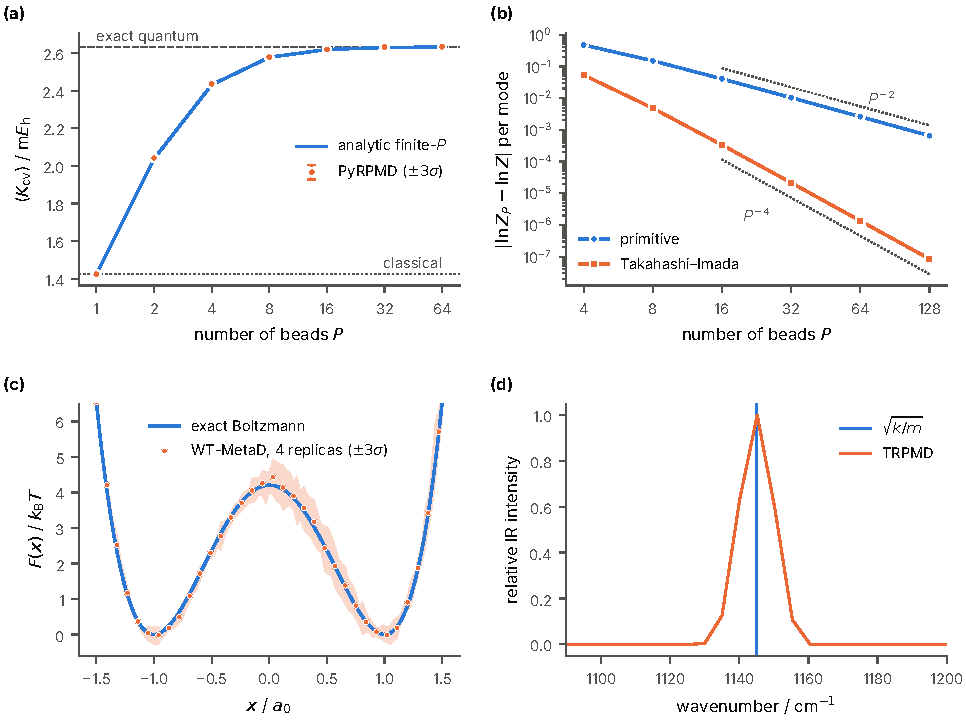
\includegraphics[width=\textwidth]{figures/equilibrium.pdf}
\caption{Equilibrium validation. (a) Centroid-virial kinetic energy of a harmonically bound proton at 300~K ($\beta\hbar\omega=3.47$) against the analytic finite-$P$ result. (b) Discretisation error of $\ln Z$ for the primitive and Takahashi--Imada actions at $\beta\hbar\omega=8$. (c) Free energy of a quartic double well from well-tempered metadynamics with frozen-bias reweighting against the bin-averaged Boltzmann result. (d) Thermostatted-RPMD infrared line of a harmonic oscillator ($P=8$) and the exact frequency.}
\label{fig:equilibrium}
\end{figure}

\subsection{Free energies, transport and spectra}

Table~\ref{tab:tutorials} collects the comparisons of four further workflows with analytic references.

\paragraph{Metadynamics} A particle in the double well $V(x)=V_0(x^{2}/a^{2}-1)^{2}$ with $V_0=0.004\,\Eh=4.2\,\kB T$ is sampled by well-tempered metadynamics (bias factor 8) on a bias grid; the bias is frozen after 10~ps and, after 2~ps of relaxation, the free energy is obtained by reweighting the remaining 18~ps of fixed-bias sampling. The profile of four independent replicas coincides with the exact Boltzmann result over the whole supported range, Fig.~\ref{fig:equilibrium}(c), and the barrier, $4.08(9)\times10^{-3}\,\Eh$, agrees with the exact bin-averaged value $3.995\times10^{-3}\,\Eh$ within $0.9\sigma$.

\paragraph{Site-to-site rate} A proton in a periodic cosine potential of period $4\,a_0$ and barrier $0.006\,\Eh$ ($6.3\,\kB T$) is treated by the full \code{site\_rate} pipeline: umbrella sampling, basin normalisation, constrained parents and recrossing children. In the classical limit the directed rate is given exactly by transition-state theory, $k_{\mathrm{TST}}=2.271\times10^{10}\,\mathrm s^{-1}$; the workflow returns $2.34(33)\times10^{10}\,\mathrm s^{-1}$ with a transmission coefficient of 1.000.

\paragraph{Diffusion} The \code{diffusion} workflow with a Markovian friction $\gamma=0.02~\mathrm{fs^{-1}}$ on a free particle reproduces the Einstein relation $D=\kB T/m\gamma$, $1.15(10)\times10^{-3}$ against $1.069\times10^{-3}$ atomic units, and identifies the ballistic regime that precedes the linear growth of the mean-square displacement.

\paragraph{Spectrum} Thermostatted RPMD with eight beads places the infrared line of a harmonic oscillator at $1145.2~\mathrm{cm^{-1}}$, Fig.~\ref{fig:equilibrium}(d), $0.2~\mathrm{cm^{-1}}$ from the exact $\sqrt{k/m}=1144.98~\mathrm{cm^{-1}}$ and well inside the $5.1~\mathrm{cm^{-1}}$ resolution of the transform; the thermostat on the internal modes leaves the centroid frequency unshifted, as it must.

\begin{table}[!htbp]
\caption{Workflow results against analytic references. $\Delta/\sigma$ is the deviation in units of the standard error over independent replicas; run times $t$ are single-core wall times of the complete workflow.}
\label{tab:tutorials}
\small
\setlength{\tabcolsep}{3pt}\begin{tabular*}{\textwidth}{@{\extracolsep{\fill}}llllrr@{}}
\toprule
Workflow & Observable & PyRPMD & Reference & $\Delta/\sigma$ & $t$/s \\
\midrule
\code{pimd} & $\langle V\rangle$, $P=16$ / $10^{-3}\Eh$ & $2.634(10)$ & $2.619$ & $1.6$ & 12 \\
\code{pimd} & $\langle K_{\mathrm{cv}}\rangle$, $P=16$ / $10^{-3}\Eh$ & $2.619(2)$ & $2.619$ & $0.0$ & 12 \\
\code{fes} (WT-MetaD) & barrier / $10^{-3}\Eh$ & $4.08(9)$ & $3.995$ & $0.9$ & 82 \\
\code{site\_rate} & $k$ / $10^{10}\,\mathrm s^{-1}$ & $2.34(33)$ & $2.271$ & $0.2$ & 111 \\
\code{diffusion} & $D$ / $10^{-3}$ a.u. & $1.15(10)$ & $1.069$ & $0.8$ & 29 \\
\code{spectroscopy} & line / $\mathrm{cm^{-1}}$ & $1145.2$ & $1144.98$ & --- & 73 \\
\bottomrule
\end{tabular*}
\end{table}

\subsection{Integrators}

Figure~\ref{fig:integrators} shows the conservation of the ring-polymer Hamiltonian for a Morse oscillator with the parameters of H$_2$ ($P=32$, 300~K), started from a thermalised configuration and propagated for 200~fs with each integrator in the fused native loop. All three schemes converge with the expected second order in the time step. At equal time step the Cayley and normal-mode splittings conserve energy about ten times more accurately than velocity Verlet, because they treat the stiff ring-polymer springs exactly or unconditionally stably; with $\Delta t=0.1$~fs the relative error of $H_P$ is $1.2\times10^{-4}$ for the Cayley scheme and $1.1\times10^{-3}$ for velocity Verlet. The discretised ring-polymer instanton of an Eckart barrier at half the crossover temperature provides an independent check of the path-integral action and its derivatives: the error of the instanton action falls from $0.081\hbar$ at $P=32$ to $0.020\hbar$ at $P=64$ and $0.0050\hbar$ at $P=128$, again second order, and the $P=128$ instanton rate agrees with the analytic continuum instanton rate to 0.5\%.

\begin{figure}[!htbp]
\centering
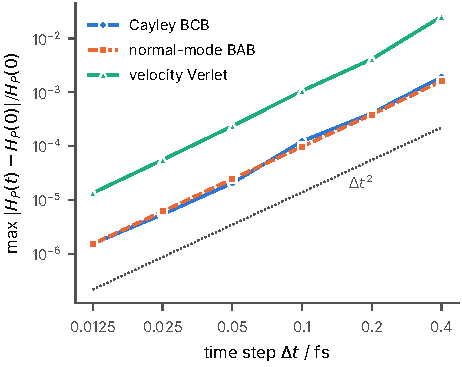
\includegraphics[width=0.55\textwidth]{figures/integrators.pdf}
\caption{Maximum relative deviation of the ring-polymer Hamiltonian over 200~fs for a 32-bead Morse oscillator at 300~K as a function of the time step.}
\label{fig:integrators}
\end{figure}

\subsection{Rate constants}
\label{sec:val-rates}

\paragraph{Two routes to one rate} We computed the thermal rate constant of a model D + H$_2\to$ DH + H exchange reaction at 1500~K with four beads by the two independent routes of Section~\ref{sec:theory}. The potential is an analytic three-body exchange surface supplied as a C library through the C ABI, so that both workflows run in the fused native loop. Each Bennett--Chandler calculation uses 66 umbrella windows on $0\le\xi\le1.05$ with two chains of 10~ps each, 1000 constrained parent configurations and 10\,000 child trajectories of 100~fs, and is repeated with four independent seeds; the direct calculation launches 20\,480 collisions from 160 parent chains in five independent runs, with $b_{\max}=4.5\,a_0$. The potential of mean force rises by $6.1\,\kB T$ between the asymptote and the barrier, Fig.~\ref{fig:rates}(a), and the transmission coefficient reaches a plateau of $\kappa=0.92$ within 40~fs, Fig.~\ref{fig:rates}(b). The results are compared in Fig.~\ref{fig:rates}(c) and Table~\ref{tab:exchange}. All 20\,480 collisions were resolved by the classifier, 231 of them reactive. The direct rate, $1.13(8)\times10^{-11}\,\rateunit$, and the Bennett--Chandler rates with umbrella integration and with MBAR, $1.11(13)$ and $1.12(13)\times10^{-11}\,\rateunit$, agree to 1\%, well within their statistical uncertainties, although the direct and the Bennett--Chandler routes share neither a sampling stage nor an estimator.

\begin{table}[!htbp]
\caption{Rate constant of the model D + H$_2$ exchange reaction at 1500~K ($P=4$) from direct RPMD and from the Bennett--Chandler (BC) factorisation with two free-energy estimators, in units of $10^{-11}\,\rateunit$. Uncertainties are standard errors over independent seeds; the two BC estimators analyse the same umbrella samples.}
\label{tab:exchange}
\small
\begin{tabular*}{\textwidth}{@{\extracolsep{\fill}}lccc@{}}
\toprule
Method & $k_{\mathrm{QTST}}$ & $\kappa$ & $k$ \\
\midrule
dRPMD, 20\,480 collisions & --- & --- & $1.13(8)$ \\
BC, umbrella integration (4 seeds) & $1.21(14)$ & $0.923(1)$ & $1.11(13)$ \\
BC, MBAR (4 seeds) & $1.21(14)$ & $0.923(1)$ & $1.12(13)$ \\
\bottomrule
\end{tabular*}
\end{table}

\begin{figure}[!htbp]
\centering
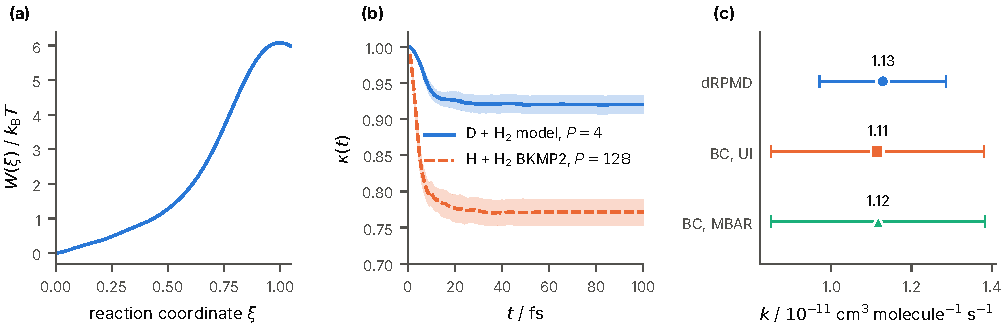
\includegraphics[width=\textwidth]{figures/rates.pdf}
\caption{Rate-constant validation. (a) Flux-weighted potential of mean force of the model D + H$_2$ reaction at 1500~K. (b) Transmission coefficient of the model reaction (band: $\pm2\sigma$) and of H + H$_2$ on the BKMP2 surface at 300~K with 128 beads (band: 95\% interval over eight independent parent chains). (c) Rate constant of the model reaction from direct RPMD and from the Bennett--Chandler factorisation with umbrella integration (UI) and MBAR; bars are $\pm2\sigma$.}
\label{fig:rates}
\end{figure}

\paragraph{H + H$_2$ on the BKMP2 surface} The hydrogen exchange reaction on the Boothroyd--Keogh--Martin--Peterson surface \cite{bkmp21996} at 300~K is the reference case of the RPMDrate article \cite{rpmrate13}, deep enough in the quantum regime that RPMD and classical rates differ by two orders of magnitude. Table~\ref{tab:h3} compares PyRPMD with the published values for the classical limit and for 128 beads. The PyRPMD entries are taken from the validation record distributed with the program, which archives inputs, seeds and raw trajectories; the potential is the original Fortran routine, attached through the C ABI and verified against its authors' test points. The classical rate reproduces the published value to 0.3\%. For 128 beads the transmission coefficient, accumulated from eight independent parent chains with paired time steps, is $\kappa=0.771$ with a 95\% interval of $[0.753,0.789]$ (published: $0.776$), Fig.~\ref{fig:rates}(b), and the rate constant is $1.968\times10^{-16}\,\rateunit$ with a 95\% interval of $[1.933,2.003]\times10^{-16}$, 0.9\% above the published $1.95\times10^{-16}$ and well inside its stated 5\% precision. The quantum-to-classical ratio of the reactant partition function that enters the normalisation was confirmed independently by a finite-$P$ radial transfer-matrix calculation, whose value lies inside the 95\% interval of the stochastic estimate.

\begin{table}[!htbp]
\caption{H + H$_2$ on the BKMP2 surface at 300~K: PyRPMD against the values published with RPMDrate \cite{rpmrate13}. Rates in $\rateunit$; brackets are 95\% intervals over independent chains.}
\label{tab:h3}
\small
\begin{tabular*}{\textwidth}{@{\extracolsep{\fill}}llll@{}}
\toprule
 & Quantity & PyRPMD & Ref.~\cite{rpmrate13} \\
\midrule
Classical ($P=1$) & $k_{\mathrm{TST}}$ & $1.553\times10^{-18}$ & $1.56\times10^{-18}$ \\
 & $\kappa$ & $0.9950$ $[0.9938,0.9962]$ & $0.994$ \\
 & $k$ & $1.545\times10^{-18}$ $[1.544,1.547]$ & $1.55\times10^{-18}$ \\
RPMD ($P=128$) & $k_{\mathrm{QTST}}$ & $2.552\times10^{-16}$ $[2.517,2.589]$ & $2.51\times10^{-16}$ \\
 & $\kappa$ & $0.771$ $[0.753,0.789]$ & $0.776$ \\
 & $k$ & $1.968\times10^{-16}$ $[1.933,2.003]$ & $1.95\times10^{-16}$ \\
\bottomrule
\end{tabular*}
\end{table}

\subsection{Electronic-structure-coupled modules}

Two further modules are validated against independent implementations in the record distributed with the program. The golden-rule proton-coupled electron-transfer rates of the \code{pcet} task agree with the pyPCET program \cite{pypcet2025} to within 0.062\% for twelve forward and reverse rates over three electrode potentials and two isotopes, and the H/D kinetic isotope effects to within 0.004\%, although the two codes solve the proton vibrational problem with different discretisations (finite differences on 1601 points against a Fourier grid of 512 points). The thermal nonadiabatic RPMD position autocorrelation function of the two-level model of Richardson and Thoss \cite{na-nrpmd2013} is reproduced with root-mean-square deviations of 0.043 and 0.026 from the published curves for one and four beads.

%% ===================================================================
\section{Performance}
\label{sec:performance}

\paragraph{Execution paths} Figure~\ref{fig:performance}(a) shows the wall time per step of the three execution paths of Section~\ref{sec:native} for a triatomic ring polymer with an analytic potential, the regime of gas-phase rate calculations in which the cost of the framework rather than of the potential is rate-limiting. The fused block advances 16 beads in $2.6~\mu$s and 128 beads in $13~\mu$s per step, against $313$ and $261~\mu$s for the NumPy reference: speed-ups of 119 and 20. The cost of the fused path grows linearly with $P$ and contains no constant interpreter overhead, which is what makes long recrossing and collision campaigns with tens of millions of steps practical on a workstation; the complete 14.5-million-step umbrella stage and 10-million-step recrossing stage of Section~\ref{sec:val-rates} take 5.6 minutes on one core. For a condensed-phase size of 512 atoms and 32 beads the fused path needs 0.49~ms per step, 13 times less than the reference. The three paths are numerically equivalent: after 1000 steps from the same initial condition, positions agree to $2\times10^{-13}\,a_0$ and momenta to $1\times10^{-11}$ atomic units.

\paragraph{Parallel scaling} Figure~\ref{fig:performance}(b) shows the speed-up of the 4096-collision dRPMD calculation of Section~\ref{sec:val-rates} with the number of worker processes. The wall time of the complete workflow, including parent thermalisation, checkpointing and analysis, falls from 61~s on one worker to 33~s on two and 20~s on four (medians of three runs), a speed-up of 3.0, and the runs return identical trajectory outcomes and the same rate constant to all sixteen digits, because random streams and checkpoints are attached to parent chains and not to workers.

\paragraph{Free-energy analysis} The streaming native MBAR solver removes the analysis as a bottleneck of large umbrella campaigns. In the benchmark recorded with the program, a converged solve for 48 umbrella states and 96\,000 samples takes 2.0~s on one core and 0.57~s on four, compared with 10.2~s for the dense NumPy/SciPy solver, while the peak memory falls from 417 to 91~MiB; free energies, weights and bootstrap barriers of the two solvers agree to $10^{-14}$.

\begin{figure}[!htbp]
\centering
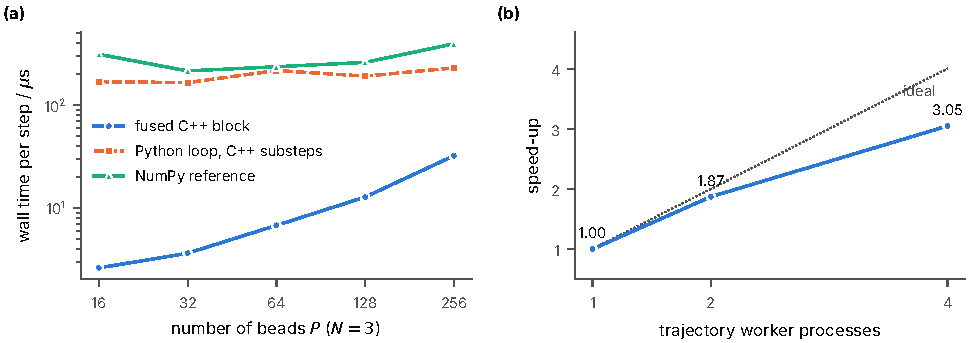
\includegraphics[width=\textwidth]{figures/performance.pdf}
\caption{Performance. (a) Wall time per RPMD step of a triatomic ring polymer on one core for the three execution paths. (b) Speed-up of a 4096-collision dRPMD calculation with the number of trajectory worker processes.}
\label{fig:performance}
\end{figure}

%% ===================================================================
\section{What the unified design delivers}
\label{sec:advantages}

\paragraph{Cross-validation inside one program} Because the Bennett--Chandler and the direct-scattering workflows share the potential interface, the integrator and the normalisation, their agreement (Table~\ref{tab:exchange}) tests the reaction coordinate, the free-energy estimator, the bimolecular prefactor, the constrained sampling and the classifier at once. The same holds for the pairs umbrella integration/MBAR, umbrella sampling/metadynamics and Cayley/normal-mode propagation, each of which can be exchanged by one line of input. A discrepancy is then a statement about sampling or about a method, not about two programs.

\paragraph{One protocol from the gas phase to surfaces and solids} The rate machinery --- flux-weighted free energy, constrained parents, paired children, joint bootstrap --- is the same for a bimolecular gas-phase reaction, for a hop between interstitial sites and for the escape of an adsorbate from a basin on a slab with fixed layers; only the normalisation differs. The centroid collective variables, the periodic boundary conditions and the fixed-atom projection are implemented once in the propagation stack and are therefore available to every workflow, including the fused native loop.

\paragraph{Native speed without loss of extensibility} A new potential, collective variable or classifier is a short Python class and runs immediately in every workflow through the compiled-substep path; a potential that is supplied as a compiled library, or a fitted surface exported through ONNX, moves the entire time loop into C++ without any change to the input. The NumPy reference implementation makes each kernel independently verifiable, and the equivalence of the three paths is part of the test suite.

\paragraph{Reproducibility by construction} Units are explicit and checked. A run directory contains everything needed to repeat the calculation and to audit it: the resolved input, the seeds, the software versions, the backend actually used, hash-verified checkpoints of every stage and the raw observations from which the reported numbers were derived. A restart cannot change the Hamiltonian, the result does not depend on the degree of parallelism, and re-analysis with different bins, estimators or bootstrap settings never calls the potential.

\paragraph{Statistical honesty as a default} The reported uncertainty of a rate constant combines the free-energy and the recrossing contributions and respects the correlation between children of one parent and between samples of one chain. Unsampled regions are masked rather than extrapolated, unresolved trajectories become explicit bounds, and a rate is withheld until its plateau is established. These conventions make results from different users of the program directly comparable.

%% ===================================================================
\section{Conclusions}
\label{sec:conclusions}

PyRPMD brings the principal observables of ring-polymer molecular dynamics --- thermal rate constants, collision outcomes, free-energy surfaces, equilibrium path-integral averages, diffusion coefficients, local escape rates and vibrational spectra --- under one input grammar, one propagation stack, one potential interface and one restart mechanism. Its fused C++17/OpenMP kernels reach microsecond time steps for gas-phase ring polymers while a NumPy twin keeps them verifiable; its free-energy toolbox couples umbrella integration, MBAR, metadynamics and OPES directly to rate theory; and its analysis layer attaches a correlation-aware uncertainty and a set of diagnostics to every result. The program reproduces analytic finite-bead results within statistical error, exhibits the expected orders of convergence of its integrators and higher-order actions, returns the same rate constant from two independent routes, and reproduces the published RPMD rate of H + H$_2$ on the BKMP2 surface to within 1\%. With adapters to \emph{ab initio} and machine-learned potentials and with modules for instantons, nonadiabatic dynamics and electrochemical proton-coupled electron transfer built on the same foundations, PyRPMD provides a single, reproducible environment for quantitative simulations of nuclear quantum effects in chemical dynamics.

\section*{Declaration of competing interest}
The authors declare that they have no known competing financial interests or personal relationships that could have appeared to influence the work reported in this paper.

%% TODO(authors): Elsevier requires a ``Declaration of generative AI and AI-assisted
%% technologies in the manuscript preparation process'' when such tools were used.
%% Add the statement that applies to this manuscript here.

\section*{Data availability}
The source code, the user manual, the inputs of all calculations reported here and the scripts and data records that regenerate the figures and tables are available in the developer's repository, \url{https://github.com/chen-yu-hao/PyRPMD}.

\section*{Acknowledgements}
%% TODO(authors): funding and computing-resource acknowledgements.

\bibliographystyle{elsarticle-num}
\bibliography{references}

\end{document}
